\section{Evaluation}
To evaluate the privacy properties of Kadcast we ran multiple simulations of
transaction broadcasting with the Kadcast algortihm. Each simulation has
the same amount of overall active nodes in the network and overall sent transactions.
We run each simulation for different percentages of spies. \\
The transactions are sent only by benign nodes, and all transactions are
randomly distributed among the sending nodes. Not each node does have to
send a transaction and some nodes may send multiple transactions. \\

First, we took a look at how the first spy estimator would perform in a standard setting,
using Kadcast with parameters used in ``real world scenarios'', i.e. a
bucket size of 20. \\

\begin{figure}
  \centering
      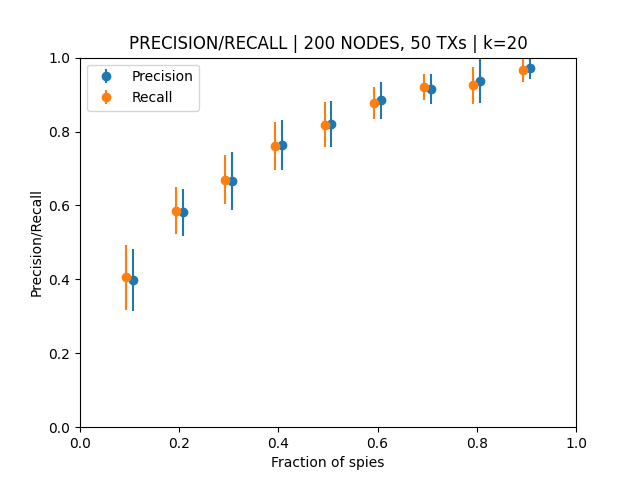
\includegraphics[width=0.5\textwidth]{figs/nodand}
  \caption{First Spy Estimator Kadcast}
  \label{fig:nodand}
\end{figure}

\begin{figure}
  \centering
      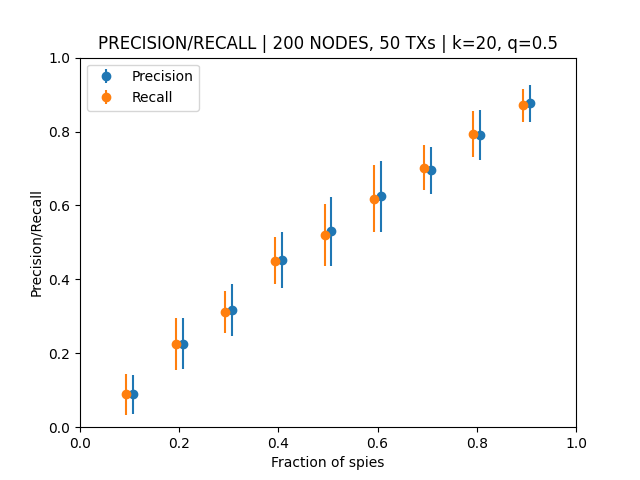
\includegraphics[width=0.5\textwidth]{figs/dand05}
  \caption{First Spy Estimator Kadcast with Dandelion}
  \label{fig:dand}
\end{figure}

The results can be seen in \ref{fig:nodand}. The figure include averaged
precision/recall values and the standard deviation of our measurements. \\
We see that the first spy estimator performs relatively well. \\
Even with an amount of as low as 20\% of spies, the attacker can
map over half of the sent transactions correctly. This is very far from
the best case scenario [TODO which is?]. \\

Just out of curiousity we wanted to test if the bucket size has any
meaningful correlation to the performance of the estimator. We therefore
repeated our experiment with common bucket sizes, the results can be
seen in [TABLE1].
Different k values did not have a positive effect on the anonymity
properties. \\

We further wanted to know if we can improve the anonymity by using dandelion spreading.
We therefore implemented a simple version of the dandelion algorithm. It
uses the ``q'' parameter as described in the original dandelion paper,
to decide at each hop if the algorithm should stop the anonymity phase
and start the broadcasting phase. The q value is the probability to leave
the anonymity phase at a hop. We did not build a Hamiltonian circuit as
described in the paper, but just used a random (loopfree) path through
the graph for each transaction. Therefore our approach is a simplified
version of dandelion, a little more akin to regular
``diffusion-by-proxy''. Nevertheless this approach has some observable
positive effects on the anonymity of our network. The result for
combining Kadcast with this simple implementation of dandelion, using
the standard parameter $q = 0.5$, can be seen in \ref{fig:dand}. Compared to
standard Kadcast spreading this is a massive improvement. \\
We ran the experiment again with different $q$ values, the results can
be seen in [TABLE2]. \\
As Dandelion only adds a constant overhead to spreading [source
dand1fanti], we think it would be a meaningful addition to Kadcast,
especially if we take the bad results we have observed in our standard
Kadcast experiments into consideration.


- auf bucket reihenfolge eingehen
- k ändern
- bucket reihenfolge ändern
- std deviation/x samples/...
